
%(BEGIN_QUESTION)
% Copyright 2010, Tony R. Kuphaldt, released under the Creative Commons Attribution License (v 1.0)
% This means you may do almost anything with this work of mine, so long as you give me proper credit

Operatører konkluderer med at en reguleringsventil har et problem, fordi spindelen står i 30\%-posisjon når sløyferegulatoren er satt til 50\% utgang i manuell modus. En tekniker går til ventilen for å feilsøke og starter med å koble multimeteret slik figuren viser:

$$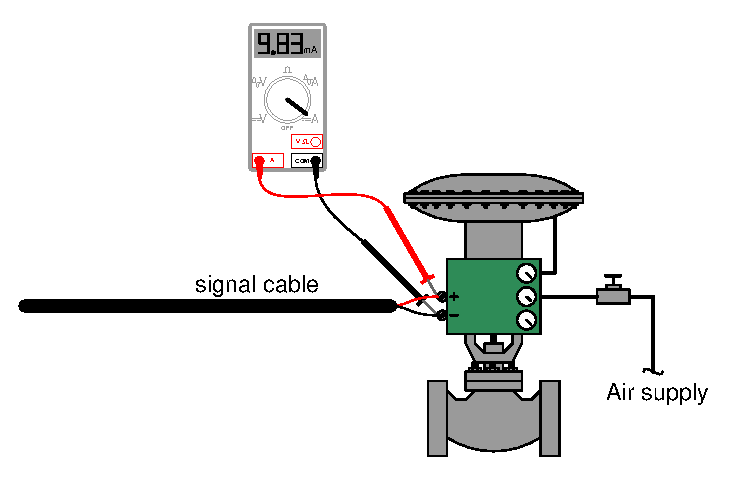
\includegraphics[width=15.5cm]{i00748x01.eps}$$

I det øyeblikket han kobler multimeteret til signalklemmene på ventilposisjoneren, lukker ventilen helt og multimeteret viser 9.83 milliampere.

\vskip 10pt

Basert på denne informasjonen: avgjør hvor feilen mest sannsynlig ligger - i {\it sløyferegulatoren}, {\it signalkablingen}, {\it posisjoneren} eller {\it aktuatoren}. Vurder også teknikerens diagnostiske strategi - ville du gjort en annen test?

\vskip 20pt \vbox{\hrule \hbox{\strut \vrule{} {\bf Forslag til sokratisk diskusjon} \vrule} \hrule}

\begin{itemize}
\item{} Hvis du var teknikeren og ikke hadde testutstyr på deg (for eksempel multimeter), hvordan ville du testet ventilen? Identifiser noen informasjonskilder tilgjengelig på denne ventilen (uten testutstyr) som er nyttige for feilsøking.
\end{itemize}

\underbar{file i00748}
%(END_QUESTION)





%(BEGIN_ANSWER)

Den åpenbare feilen i teknikerens test er at han koblet amperemeteret i {\it parallell} når det skulle vært koblet i {\it serie}.

%(END_ANSWER)





%(BEGIN_NOTES)

Slik testen står, forteller den oss ikke så mye annet enn at regulatoren sannsynligvis ikke er feilkilden, og at kablingen sannsynligvis heller ikke er det.

\vskip 10pt

Grunnen til at amperemeteret ikke viser 12 mA (tilsvarer 50\%) er at parallellkoblingen mot posisjoneren deler strømmen mellom de to grenene, slik at amperemeteret ikke måler hele strømmen fra regulatoren.

\vskip 10pt

Siden prosentekvivalenten av 9.83 mA i et 4-20 mA-område er høyere enn ventilspindelens posisjon på 30\%, kan vi trygt konkludere med at dette ikke er regulatorfeil. Hvis regulatoren var feilen, ville målt strøm vært maksimalt 8.8 mA (30\%). Kabelfeil er også mindre sannsynlig, fordi en slik feil oftest ville være enten brudd eller kortslutning, og da ville målt strøm i praksis vært nær null.

%INDEX% Sluttkontrollelementer: feilsøking

%(END_NOTES)


